
%(BEGIN_QUESTION)
% Copyright 2011, Tony R. Kuphaldt, released under the Creative Commons Attribution License (v 1.0)
% This means you may do almost anything with this work of mine, so long as you give me proper credit

In many microwave radio systems, hollow rectangular tubes known as {\it waveguides} are often used in lieu of cables to serve as transmission lines between the transceiver and the antenna.  These hollow metal tubes acts as ``pipes'' to convey GHz-range electromagnetic waves with great efficiency, far exceeding the efficiency of coaxial cables:

$$\includegraphics[width=15.5cm]{i00791x01.eps}$$

The following table shows a comparison between RG-49/U waveguide and RG-9/U flexible cable:

% No blank lines allowed between lines of an \halign structure!
% I use comments (%) instead, so that TeX doesn't choke.

$$\vbox{\offinterlineskip
\halign{\strut
\vrule \quad\hfil # \ \hfil & 
\vrule \quad\hfil # \ \hfil & 
\vrule \quad\hfil # \ \hfil \vrule \cr
\noalign{\hrule}
%
% First row
{\bf Parameter} & {\bf RG-49/U waveguide} & {\bf RG-9/U coaxial cable} \cr
%
\noalign{\hrule}
%
% Another row
{\it External dimensions} & 2 inch $\times$ 1 inch & 0.420 inch diameter \cr
%
\noalign{\hrule}
%
% Another row
{\it Dielectric} & air & polyethylene (plastic) \cr
%
\noalign{\hrule}
%
% Another row
{\it Weight} & 1.4 lb per foot & 0.15 lb per foot \cr
%
\noalign{\hrule}
%
% Another row
{\it Attenuation at $f$ = 5 GHz} & 0.011 dB per foot & 0.23 dB per foot \cr
%
\noalign{\hrule}
%
% Another row
{\it Power rating} & 1.2 MW & 66 W \cr
%
\noalign{\hrule}
} % End of \halign 
}$$ % End of \vbox

Suppose an RG-49/U waveguide is used to transfer RF energy from a 300 watt radar transceiver to a dish antenna.  Calculate the RF power (in watts) available at the antenna, assuming the waveguide is 8 feet long and that there are no other power losses between the transceiver and the antenna.

\vskip 10pt

Now suppose that radar transceiver's power is increased to 800 watts.  Calculate the RF power (in watts) available at the antenna, assuming the same waveguide length.

\vskip 10pt

Now suppose that radar transceiver's power is increased to 3 kilowatts.  Calculate the RF power (in watts) available at the antenna, assuming the same waveguide length.

\vskip 10pt

Does the waveguide power loss remain constant as transmitter power increases, or does it change with the amount of transmitted power?  How does the ``lost'' RF energy manifest itself through the waveguide (given that the Law of Energy Conservation tells us energy cannot be created or destroyed)?

\vskip 20pt \vbox{\hrule \hbox{\strut \vrule{} {\bf Suggestions for Socratic discussion} \vrule} \hrule}

\begin{itemize}
\item{} Explain why the waveguide shown has such a greater power rating than the coaxial cable, based on their respective dB/foot loss ratings.
\item{} Why aren't waveguides used for all GHz-frequency radio applications, given that their power losses are so much less than the losses exhibited by coaxial cable?
\item{} For those who have studied level measurement technologies, explain how the concept of a {\it waveguide} relates to guided-wave radar (GWR) level transmitters.
\item{} Is is possible for a waveguide to experience {\it reflected signals} as in the case of improperly terminated transmission line cables?  Why or why not?
\end{itemize}

\underbar{file i00791}
%(END_QUESTION)





%(BEGIN_ANSWER)

$P_{antenna}$ = 293.98 W at a transmitted power of 300 W.

\vskip 10pt

$P_{antenna}$ = 783.95 W at a transmitted power of 800 W.

\vskip 10pt

$P_{antenna}$ = 2.9398 kW at a transmitted power of 3 kW.

%(END_ANSWER)





%(BEGIN_NOTES)

An RG-49/U waveguide 8 feet in length will exhibit a total power attenuation of:

$$(8 \hbox{ ft}) (-0.011 \hbox{ dB/ft}) = -0.088 \hbox{ dB}$$

This equates to an attenuation (expressed as a ratio) of:

$$10^{-0.088 \over 10} = 0.97994$$

Thus, the waveguide conveys 97.994\% of its input power to the antenna.

\vskip 10pt

Here are the calculations of power delivered to the antenna, at different transmitter power levels:

$$(300 \hbox{ W}) (0.97994) = 293.98 \hbox{ W}$$

$$(800 \hbox{ W}) (0.97994) = 783.95 \hbox{ W}$$

$$(3000 \hbox{ W}) (0.97994) = 2939.82 \hbox{ W}$$

\vskip 10pt

Power loss increases with incident (transmitter) power.  This loss is typically manifested in the form of heat, although it is possible for some of the energy to radiate away from the waveguide (or cable) in the form of electromagnetic waves, especially if there are any gaps in the waveguide flange seals.

\vskip 10pt

Data for the waveguide/cable comparison came from the {\it Electronics Manual for Radio Engineers}, first edition, by Vin Zeluff and John Markus (1949), page 448.

















\vfil \eject

\noindent
{\bf Prep Quiz:}

A {\it waveguide} is:

\begin{itemize}
\item{} A tool used to properly align directional radio antennas for optimum reception
\vskip 5pt 
\item{} A hollow metal structure used to convey RF energy, like a transmission line
\vskip 5pt 
\item{} A metal rod providing mechanical rigidity for a telescoping radio antenna
\vskip 5pt 
\item{} An instrument designed to measure radio signal strength in one direction
\vskip 5pt 
\item{} A device used to calm the surface of a liquid for better level measurement
\vskip 5pt 
\item{} One of the elements of a Yagi antenna, used to make it more directional
\end{itemize}


\vfil \eject

\noindent
{\bf Prep Quiz:}

Calculate the amount of RF power available at a transmitting radio antenna (in watts) if the transmitter outputs 30 watts and the connecting cable in between the transmitter and the antenna has a total loss of -1.3 dB.

\begin{itemize}
\item{} 1.5 watts
\vskip 5pt 
\item{} 34.2 watts
\vskip 5pt 
\item{} 22.24 watts
\vskip 5pt 
\item{} 26.33 watts
\vskip 5pt 
\item{} 28.7 watts
\vskip 5pt 
\item{} 31.3 watts
\end{itemize}


%INDEX% Electronics review: decibel power calculations
%INDEX% Electronics review: waveguides

%(END_NOTES)


